
\begin{aufgabe}
Geben Sie für die vier folgenden Weg-Zeit-Diagramme an, ob die Geschwindigkeit $v_1$ 
zum Zeitpunkt $t_1$ grösser, kleiner oder gleich der Geschwindigkeit $v_2$ zum Zeitpunkt $t_2$ ist.\\

\begin{minipage}{0.5\textwidth}
%\input{./Mechanik/weg-zeit-diagramm_a.pgf}
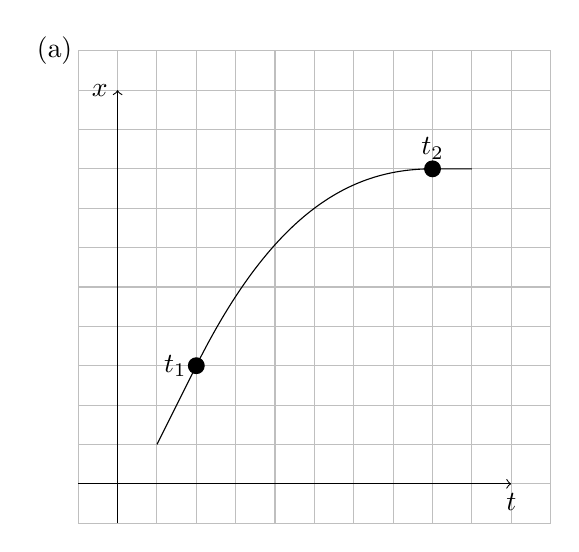
\begin{tikzpicture}
\draw[step=0.5cm,lightgray] (-0.5,-0.5) grid (5.5,5.5);

\draw  (-0.8,5.5) node {(a)};

%begin Koordinatensystem
%x-achse
\coordinate (C1) at (-0.5,0);
\coordinate [label=below:$t$] (C2) at (5,0);
\draw  [->] (C1)--(C2);

%y-achse
\coordinate (C3) at (0,-0.5);
\coordinate [label=left:$x$] (C4) at (0,5);
\draw [->] (C3)--(C4);
%end Koordinatensystem



\coordinate (P1) at (0.5,0.5);
\coordinate [label=$t_2$] (P3) at (4,4);
\coordinate [label=left:$t_1$] (P2) at (1,1.5);
\draw  [fill] (P2) circle (0.1);
\draw [fill] (P3) circle (0.1);

\draw (P1)--(P2)  .. controls (2,3.5) and (3.0,4) .. (P3)--+(0.5,0);

\end{tikzpicture}

\end{minipage}
\begin{minipage}{0.5\textwidth}
%\input{./Mechanik/weg-zeit-diagramm_b.pgf}
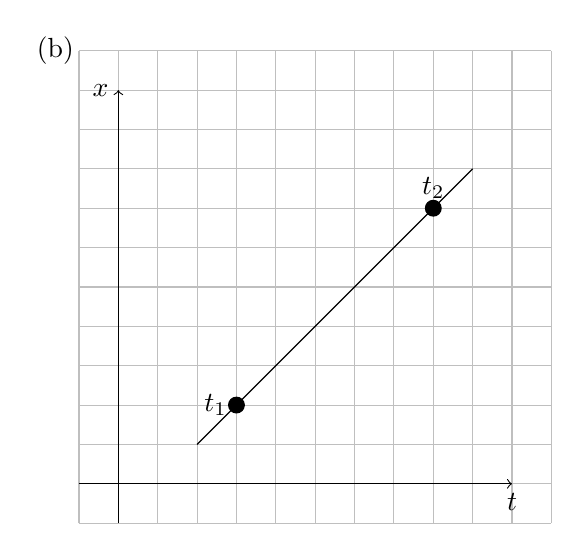
\begin{tikzpicture}
\draw[step=0.5cm,lightgray] (-0.5,-0.5) grid (5.5,5.5);

\draw  (-0.8,5.5) node {(b)};

%begin Koordinatensystem
%x-achse
\coordinate (C1) at (-0.5,0);
\coordinate [label=below:$t$] (C2) at (5,0);
\draw  [->] (C1)--(C2);

%y-achse
\coordinate (C3) at (0,-0.5);
\coordinate [label=left:$x$] (C4) at (0,5);
\draw [->] (C3)--(C4);
%end Koordinatensystem




\coordinate [label=$t_2$] (P3) at (4,3.5);
\coordinate [label=left:$t_1$] (P2) at (1.5,1);
\draw  [fill] (P2) circle (0.1);
\draw [fill] (P3) circle (0.1);


\draw (1,0.5)--(4.5,4);
\end{tikzpicture}

\end{minipage}

\begin{minipage}{0.5\textwidth}
%\input{./Mechanik/weg-zeit-diagramm_c.pgf}

\begin{tikzpicture}
%\usetikzlibrary{calc,intersections,through,backgrounds}
\draw[step=0.5cm,lightgray] (-0.5,-0.5) grid (5.5,5.5);

\draw  (-0.8,5.5) node {(c)};

%begin Koordinatensystem
%x-achse
\coordinate (C1) at (-0.5,0);
\coordinate [label=below:$t$] (C2) at (5,0);
\draw  [->] (C1)--(C2);

%y-achse
\coordinate (C3) at (0,-0.5);
\coordinate [label=left:$x$] (C4) at (0,5);
\draw [->] (C3)--(C4);
%end Koordinatensystem



\coordinate (P1) at (0.5,4.5);
\coordinate (P2) at (1.5,0.5);
\coordinate (P3) at (2.5,0.5);
\coordinate (P4) at (4.5,1.5);




\draw [name path = C] (P1) .. controls (P2) and (P3) .. (P4);

%erster punkt
\node (D1) [name path=D1, circle, minimum size=1cm ] at (P1) {};
\path [name intersections = {of=C and D1, by=F1}];
\draw [fill] (F1) circle (0.1);
\draw (F1) node [right] {$t_1$};

%zweiter punkt
\node (D2) [name path=D2, circle, minimum size=1cm] at (P4) {};
\path [name intersections = {of=C and D2, by=F2}];
\draw[fill] (F2) circle (0.1);
\draw (F2) node [above]  {$t_2$};

\end{tikzpicture}
\end{minipage}
\begin{minipage}{0.5\textwidth}
%\input{./Mechanik/weg-zeit-diagramm_d.pgf}

\begin{tikzpicture}
%\usetikzlibrary{calc,intersections,through,backgrounds}
\draw[step=0.5cm,lightgray] (-0.5,-0.5) grid (5.5,5.5);

\draw  (-0.8,5.5) node {(d)};

%begin Koordinatensystem
%x-achse
\coordinate (C1) at (-0.5,0);
\coordinate [label=below:$t$] (C2) at (5,0);
\draw  [->] (C1)--(C2);

%y-achse
\coordinate (C3) at (0,-0.5);
\coordinate [label=left:$x$] (C4) at (0,5);
\draw [->] (C3)--(C4);
%end Koordinatensystem



\coordinate (P1) at (0.5,2.5);
\coordinate (P2) at (1.5,3.5);
\coordinate (P3) at (2.5,4.5);
\coordinate (P4) at (4.5,0.5);




\draw [name path = C] (P1) .. controls (P2) and (P3) .. (P4);

%erster punkt
\node (D1) [name path=D1, circle, minimum size=1cm ] at (P1) {};
\path [name intersections = {of=C and D1, by=F1}];
\draw [fill] (F1) circle (0.1);
\draw (F1) node [above] {$t_1$};

%zweiter punkt
\node (D2) [name path=D2, circle, minimum size=1cm] at (P4) {};
\path [name intersections = {of=C and D2, by=F2}];
\draw[fill] (F2) circle (0.1);
\draw (F2) node [right]  {$t_2$};

\end{tikzpicture}
\end{minipage}


\kloesung{a) $v_1 > v_2 \qquad |v_1| > |v_2|$\\b) $v_1 = v_2 \qquad |v_1| = |v_2|$\\c) $v_1 < v_2 \qquad |v_1| > |v_2|$\\d) $v_1 > v_2 \qquad |v_1| < |v_2|$}



\begin{loesung}
	\begin{itemize}
		\item[a)] $v_1 > v_2 \qquad |v_1| > |v_2|$
		\item[b)] $v_1 = v_2 \qquad |v_1| = |v_2|$ 
		\item[c)] $v_1 < v_2 \qquad |v_1| > |v_2|$
		\item[d)] $v_1 > v_2 \qquad |v_1| < |v_2|$
	\end{itemize}
\end{loesung}

\end{aufgabe}
